% Options for packages loaded elsewhere
\PassOptionsToPackage{unicode}{hyperref}
\PassOptionsToPackage{hyphens}{url}
%
\documentclass[
]{article}
\usepackage{lmodern}
\usepackage{amssymb,amsmath}
\usepackage{ifxetex,ifluatex}
\ifnum 0\ifxetex 1\fi\ifluatex 1\fi=0 % if pdftex
  \usepackage[T1]{fontenc}
  \usepackage[utf8]{inputenc}
  \usepackage{textcomp} % provide euro and other symbols
\else % if luatex or xetex
  \usepackage{unicode-math}
  \defaultfontfeatures{Scale=MatchLowercase}
  \defaultfontfeatures[\rmfamily]{Ligatures=TeX,Scale=1}
\fi
% Use upquote if available, for straight quotes in verbatim environments
\IfFileExists{upquote.sty}{\usepackage{upquote}}{}
\IfFileExists{microtype.sty}{% use microtype if available
  \usepackage[]{microtype}
  \UseMicrotypeSet[protrusion]{basicmath} % disable protrusion for tt fonts
}{}
\makeatletter
\@ifundefined{KOMAClassName}{% if non-KOMA class
  \IfFileExists{parskip.sty}{%
    \usepackage{parskip}
  }{% else
    \setlength{\parindent}{0pt}
    \setlength{\parskip}{6pt plus 2pt minus 1pt}}
}{% if KOMA class
  \KOMAoptions{parskip=half}}
\makeatother
\usepackage{xcolor}
\IfFileExists{xurl.sty}{\usepackage{xurl}}{} % add URL line breaks if available
\IfFileExists{bookmark.sty}{\usepackage{bookmark}}{\usepackage{hyperref}}
\hypersetup{
  hidelinks,
  pdfcreator={LaTeX via pandoc}}
\urlstyle{same} % disable monospaced font for URLs
\usepackage{longtable,booktabs}
% Correct order of tables after \paragraph or \subparagraph
\usepackage{etoolbox}
\makeatletter
\patchcmd\longtable{\par}{\if@noskipsec\mbox{}\fi\par}{}{}
\makeatother
% Allow footnotes in longtable head/foot
\IfFileExists{footnotehyper.sty}{\usepackage{footnotehyper}}{\usepackage{footnote}}
\makesavenoteenv{longtable}
\usepackage{graphicx}
\makeatletter
\def\maxwidth{\ifdim\Gin@nat@width>\linewidth\linewidth\else\Gin@nat@width\fi}
\def\maxheight{\ifdim\Gin@nat@height>\textheight\textheight\else\Gin@nat@height\fi}
\makeatother
% Scale images if necessary, so that they will not overflow the page
% margins by default, and it is still possible to overwrite the defaults
% using explicit options in \includegraphics[width, height, ...]{}
\setkeys{Gin}{width=\maxwidth,height=\maxheight,keepaspectratio}
% Set default figure placement to htbp
\makeatletter
\def\fps@figure{htbp}
\makeatother
\setlength{\emergencystretch}{3em} % prevent overfull lines
\providecommand{\tightlist}{%
  \setlength{\itemsep}{0pt}\setlength{\parskip}{0pt}}
\setcounter{secnumdepth}{-\maxdimen} % remove section numbering
\usepackage{color}
\usepackage{soulutf8}

\author{}
\date{}

\begin{document}

\hypertarget{header-n1203}{%
\section{Análisis de Datos Ómicos PEC\_1}\label{header-n1203}}

Iago Lastra Rodríguez - Abril 2020

\tableofcontents

\hypertarget{header-n1207}{%
\subsection{Abstract}\label{header-n1207}}

\hypertarget{header-n1208}{%
\subsection{Objetivos}\label{header-n1208}}

Aunque los inhibidores de factores de necrosis
tumoral\href{https://es.wikipedia.org/wiki/Factor_de_necrosis_tumoral}{TNF}
son \href{https://www.ncbi.nlm.nih.gov/pubmed/15370396}{utilizados en el
tratamiento de enfermedades inflamatorias crónicas} no existe demasiada
información acerca de cómo pueden afectar estos tratamientos al
funcionamiento normal del sistema nervioso central.

En este trabajo se analizarán Microarrays de ARN para buscar diferencias
estadísticamente significativas entre muestras sin tratar (WT) y
muestras sometidas a tratamientos de inhibición de TNF.

\hypertarget{header-n1211}{%
\subsection{Materiales y Métodos}\label{header-n1211}}

Este trabajo se basa en estúdio de comparación de grupos (class
comparison) donde se han tomado muestras correspondientes al dia 13.5 de
la fase embrionaria (E13.5) al séptimo día de vida (P7) y en adultos de
2 y 4 meses de vida (A2 y A4 respectivamente) de un grupo de control
(WT) de ratones \href{https://en.wikipedia.org/wiki/C57BL/6}{C57BL/6} y
un segundo grupo de ratones tratados (TNF-/-).

Los microarrays utilizados son del modelo GeneChip Mouse Gene 1.0 ST
Array de Affymetrix que según su especificación contienen
aproximadamente 25 sondas (probes) diseñadas para cubrir 28,853 genes
bien conocidos y anotados.

\hypertarget{header-n1214}{%
\subsubsection{Procedimiento de trabajo}\label{header-n1214}}

En un primer paso se analizaron gráficamente los archivos .CEL buscando
posibles errores en los datos. Aunque tanto el histograma como el
boxplot mostraron datos bastante uniformes se realizó una comprobación
adicional utilizando el paquete \texttt{arrayQualityMetrics} para
verificar que los datos no contenían errores.

\begin{figure}
\centering
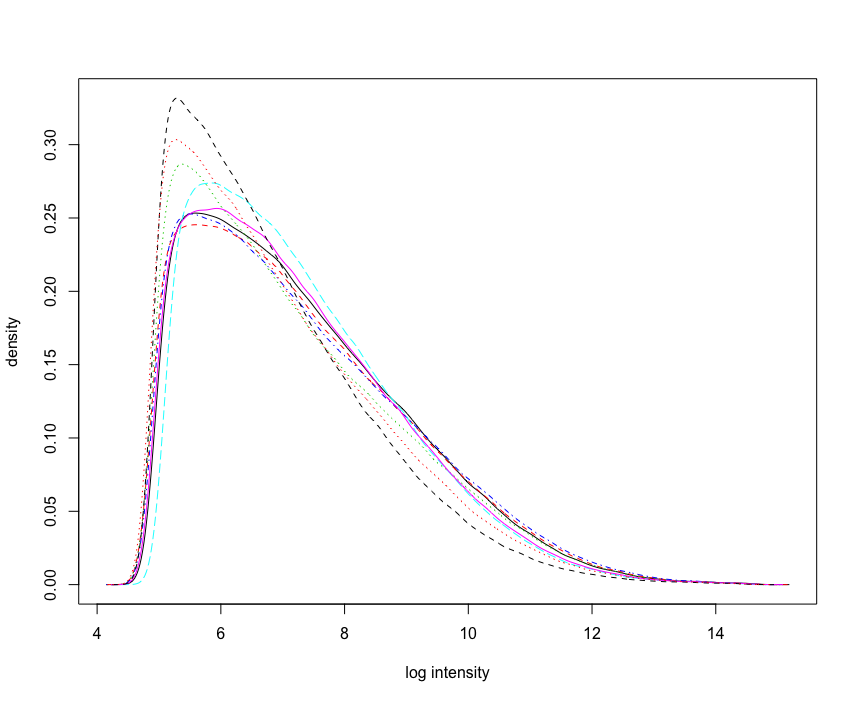
\includegraphics{/Users/iagolast/Workspace/personal/ADO_PEC_1/img/raw_data_histogram.png}
\caption{}
\end{figure}

\begin{figure}
\centering
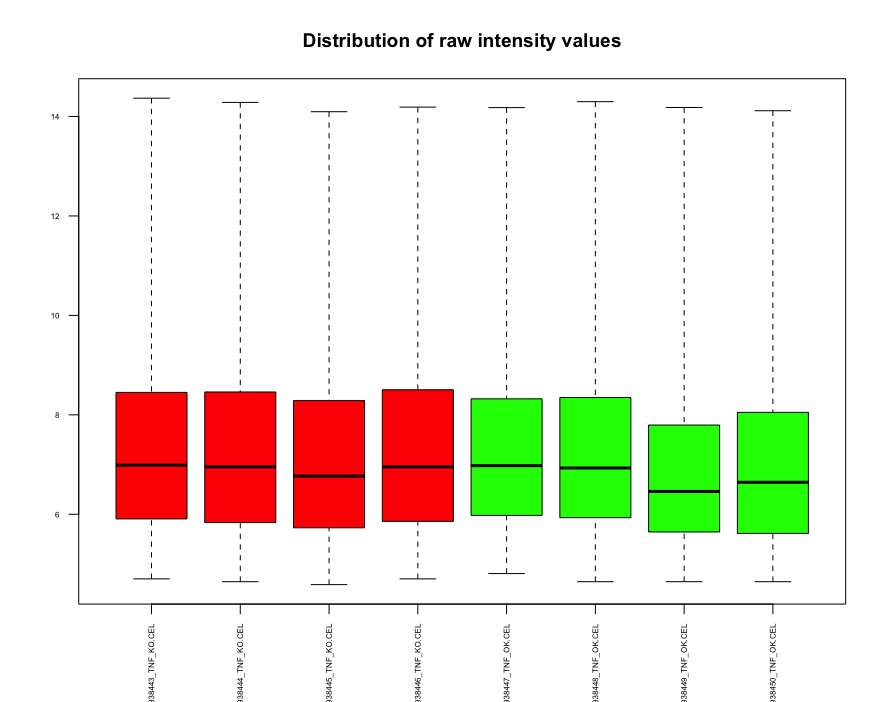
\includegraphics{/Users/iagolast/Workspace/personal/ADO_PEC_1/img/raw_data_boxplot.png}
\caption{}
\end{figure}

\textbf{Normalización}

Para poder realizar un análisis de la expresión diferencial de los datos
es necesario transformar los datos para que sean comparables entre sí.

Esta transformación se ha realizado utilizado el algorimo Robust
Multichip Analysis (RMA) que a grandes rasgos corrige el ruido de
forndo, normaliza los datos y realiza una estimación final de la
intensidad.

Una vez obtenidos los datos normalizados se repite el control de calidad
sobre los mismos.

\textbf{Filtrado}

Para eliminar el ruido consecuencia de la variabilidad aleatoria en los
datos se ha utilizado la función \texttt{nsFilter} del paquete
\texttt{genefilter} para descartar los genes con menor variabilidad.

\textbf{Selección de genes diferencialmente expresados}

Para escoger los genes se han utilizado dos aproximaciones estadísticas.

Por un lado se ha realizado un t-test (\texttt{rowttest}) y por otro se
ha utilizado el método de Smyth (\texttt{limma}) visto en prácticas
previas.

Dado el grán número de genes que se tienen en cuenta se ha aplicado una
corrección sobre el p-valor de los genes seleccionados mediante el
t-test. Dado que estamos dispuestos a asumir una cantidad de falsos
positivos a cambio de maximizar los genes candidatos para el posterior
análisis de significación biológica, se ha optado por el método de
Benjamini \& Hochber.

Los genes seleccionados y su significación han sido.

\begin{longtable}[]{@{}lr@{}}
\toprule
SYMBOL & BH\tabularnewline
\midrule
\endhead
9430060I03Rik & 0.0431307\tabularnewline
Gm10787 & 0.0431307\tabularnewline
Gm10024 & 0.0431307\tabularnewline
Gm11696 & 0.0431307\tabularnewline
Dnmt3aos & 0.0491421\tabularnewline
Gm10782 & 0.0431307\tabularnewline
BC025933 & 0.0431307\tabularnewline
Gm10536 & 0.0431307\tabularnewline
Gm10532 & 0.0431307\tabularnewline
Gm10857 & 0.0431307\tabularnewline
Gm10804 & 0.0491421\tabularnewline
Gm10714 & 0.0431307\tabularnewline
Oog3 & 0.0431307\tabularnewline
Gm10369 & 0.0431307\tabularnewline
Gm10445 & 0.0491421\tabularnewline
Gm10610 & 0.0431307\tabularnewline
Fam129c & 0.0431307\tabularnewline
Gm10655 & 0.0431307\tabularnewline
\bottomrule
\end{longtable}

Por otra parte, los genes seleccionados mediante regresión lineal son:

\begin{longtable}[]{@{}llr@{}}
\toprule
\textbf{PROBE\_ID} & SYMBOL & adj.P.Val\tabularnewline
\midrule
\endhead
10423836 & Cthrc1 & 0.0311910\tabularnewline
10418205 & Plac9b & 0.0311910\tabularnewline
10566326 & Trim12a & 0.0311910\tabularnewline
10471675 & Glo1 & 0.0311910\tabularnewline
10398432 & Mir377 & 0.0311910\tabularnewline
10572130 & Lpl & 0.0361161\tabularnewline
10412394 & Nnt & 0.0410250\tabularnewline
\bottomrule
\end{longtable}

Con esto se ha podido realizar un análisis enrich dando como resultado
las siguientes vías:

\begin{figure}
\centering
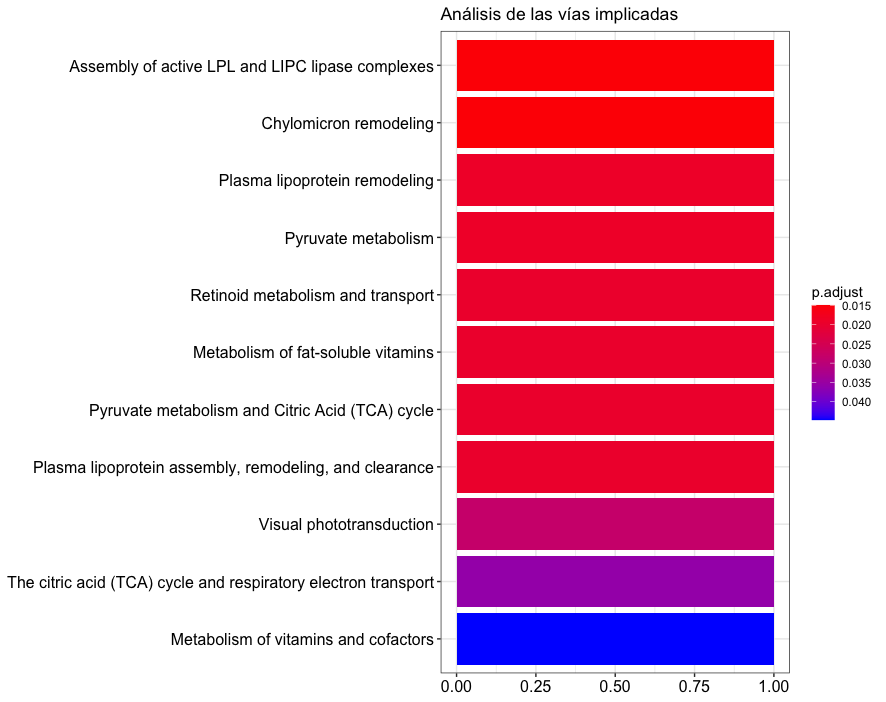
\includegraphics{/Users/iagolast/Workspace/personal/ADO_PEC_1/img/enrich.png}
\caption{}
\end{figure}

\hypertarget{header-n1363}{%
\subsection{Resultados}\label{header-n1363}}

\hypertarget{header-n1364}{%
\subsection{Discusión}\label{header-n1364}}

\begin{itemize}
\item
  Los dos métodos dan vias diferentes que a la vez son diferentes a las
  del propio paper.
\end{itemize}

\hypertarget{header-n1366}{%
\subsection{Apéndice}\label{header-n1366}}

\hl{TODO: Link al repo}

\textbf{Estudio:}
https://www.ncbi.nlm.nih.gov/geo/query/acc.cgi?acc=GSE134178

\textbf{ID\_DATA}: GSE134178

\textbf{BioProject:} https://www.ncbi.nlm.nih.gov/bioproject/PRJNA554146

Visualizar datos enrichment:

https://yulab-smu.github.io/clusterProfiler-book/chapter12.html

\end{document}
